\chapter{Transiciones de fase: Estabilidad}

Para analizar la dinámica del sistema de competencia de especies se van a considerar redes aleatorias con pesos, lo que en el capítulo pasado llamamos como \textit{matriz de incidencias} de 25, 50 y 100 nodos respectivamente. Cada una de las entradas de la matriz de incidencias representa un enlace entre nodos y su magnitud de interaccion que de acuerdo con su signo puede ser de ``cooperación" o de ``competencia". Por el hecho de tomar en cuenta distribuciones normales para los pesos de cada entrada de la matriz de adyacencia asociada a la red aleatoria, es posible obtener un $50\%$ de probabilidad de que sea positivo y $50\%$ de que sea negativo, al tener varios coeficientes de cooperación nos orilla a que existan especies que se beneficien tanto de esto que puede que rebasen la capacidad de carga del sistema, y no será por un tema de recursos en el sistema sino por el tema de la misma cooperación que hace que las especies puedan encontrar estabilidad en un punto mayor.
\\
\\
Esto se verá una vez que veamos como son las series de tiempo de los sistemas. Por lo pronto hablemos de los parámetros empleados para la resolución. Con el fin de tener el mayor número de parámetros controlados, se han definido constantes para cada uno de los cálculos realizados, en concreto se definió una tasa de crecimiento $r=2$, una capacidad de carga de $K=5$ para cada especie, se ha integrado para un intervalo discreto de tiempo de $t\in[0,50]$ con un paso de integración $h=0.01$. Por último, los únicos parámetros que si podían variar para realizar el análisis exploratorio son $N$ en número de especies, $\sigma$ la desviación estándar y $p$ la probabilidad.\\
\\
A grandes rasgos lo que representa cada uno de estos 3 parámetros variables es lo siguiente: $N$ simplemente define el tamaño del sistema, entre más grande sea el sistema es cada vez menos probable que el sistema sea estable por la cantidad de interacciones que se encuentran disponibles; por otro lado la $p$ nos define la cantidad de enlace en la red que esta representada con las interacciones entre especies, por su parte entre más grande sea la $p$ es menos probable que sea estable el sistema; por último la $\sigma$ representa la fuerza de las interacciones entre especies, que tan predominante o cooperativo (dependiendo del signo) es la especie $j$ con la especie $i$, entre más fuertes sean las interacciones es menos probable que el sistema sea estable. Por lo tanto la estabilidad esta dada en función de la magnitud de estos 3 parámetros y su relación entre ellos tal y como lo establece May en su trabajo [\footnote{agregar cita}].\\
\\
Si se considerara un sistema de competencia puro en donde cada una de las entradas de la matriz de incidencias fuera positiva, el sistema seguiría fielmente el comportamiento logístico de sus ecuaciones impidiendo que puedan crecer más alla de su capacidad de carga. De hecho es probable que sus puntos de equilibrio se encuentren en el intervalo de $[0,K]$. En la Fig. (\ref{fig:Seriesdetiempopostiva}) se ha integrado un sistema de 100 ecuaciones para una matriz de incidencias con $p=1$, es decir, que tiene un número máximo de enlaces/interacciones. Se ha comenzado con una condición inicial en el vector 1 100-dimensional con tasa de crecimiento $r=2$ y capacidad de carga $K=5$. 
\begin{figure}[h!]
	\centering
	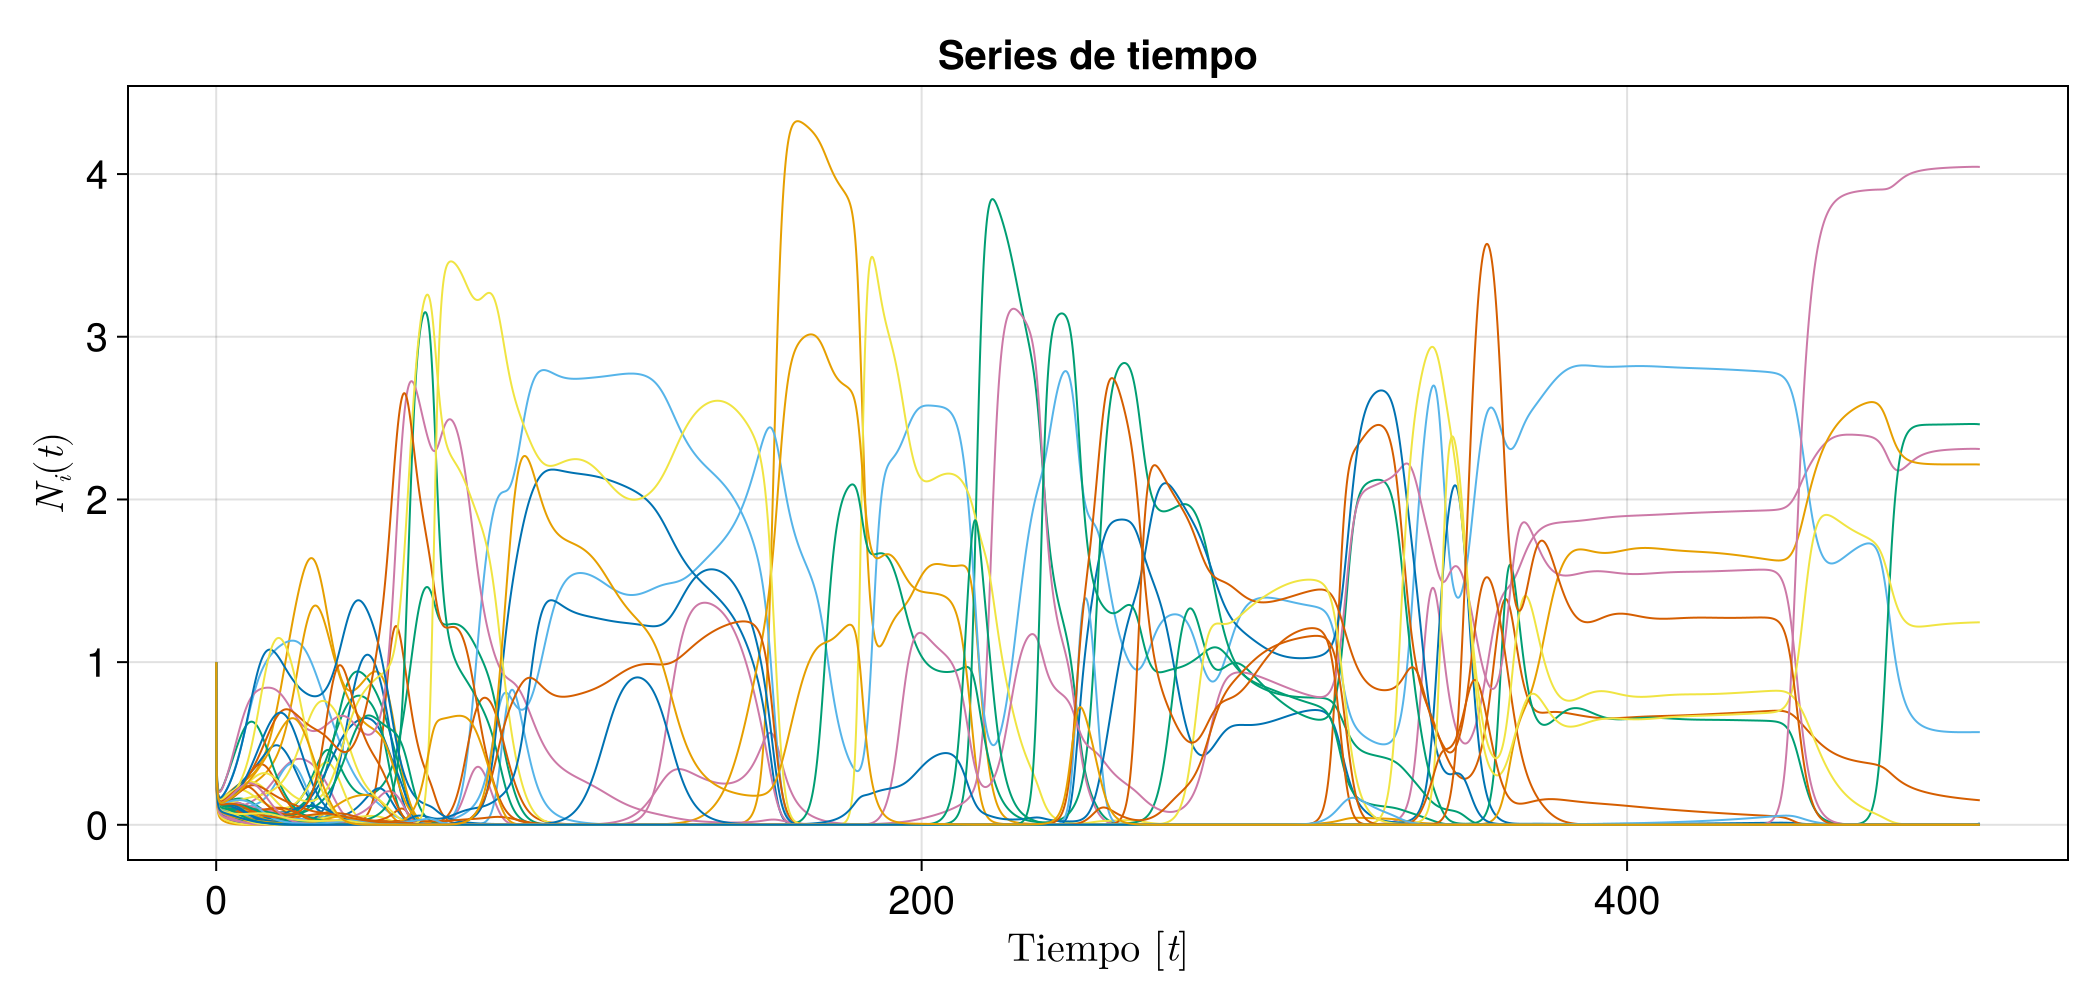
\includegraphics[scale=0.23]{../Imagenes/Seriesdetiempopositiva}
	\caption{Series de tiempo para el sistema de competencia de especies. Se emplea una matriz de incidencias de $100\times 100$cuyas entradas son de una distribución uniforme en el intervalo [0,1]. En este caso particular no se considera a $\sigma$, solamente el tamaño de la red con $p=1.0$, es decir que es una red con el número máximo de enlaces posibles. En este caso la dinámica no sobrepasa la capacidad de carga puesto que las 100 especies se encuentran compitiendo y obedecen fielmente al comportamiento logístico.}
	\label{fig:Seriesdetiempopostiva}
\end{figure}
El resultado muestra una dinámica caótica que eventualmente va tendiendo poco a poco a su punto de equilibrio (para $t\to\infty$), lo que asegura que el sistema es estable. Para este caso particular en donde consideramos una matriz de incidencias con entradas aleatorias y positivas, se estima que nunca podrá ser inestable debido a que los términos de la suma de la ecuación \ref{eqn:LK} siempre serán negativos, por tanto sus interacciones siempre se están restando y aunque en algunos instantes exista crecimiento, las ecuaciones lo restringen hasta su capacidad de carga. Realizar el análisis de esta tesis con este tipo de matrices no hubiera sido tan provechoso, pues lo que se quiere explorar es la estabilidad de los sistemas de Lotka-Volterra en presencia de competencia y cooperación.\\
\\
Como ya se ha mencionado, cuando se consideran términos de cooperación cuyos coeficientes en la matriz de incidencias son negativos se tiene la capacidad de que la dinámica pueda sobrepasar la capacidad de carga. Volviendo a la Ec. (\ref{eqn:LK}), cuando la $\alpha_{ij}<0$ y con el signo $(-)$ de la suma, hace que se vuelvan positivo y ello significa un crecimiento significativo en la población $i$. En los casos en donde consideramos una matriz de incidencias mapeada con una distribución normal centrada en cero, ahora se deben de manejar con cuidado los parámetros $N$, $\sigma$ y $p$ para que en su conjunción puedan dar lugar a sistemas estables o de lo contrario inestables.
\begin{figure}[h!]
	\centering
	\includegraphics[scale=0.23]{../Imagenes/Series de Tiempo LK100}
	\caption{(\textbf{A}) Series de tiempo para el sistema de especies en competencia asociada a una matriz de incidencias de $100\times100$, con $\sigma=0.2$ y $p=0.35$. (\textbf{B}) Series de tiempo para el sistema de especies en competencia asociada a una matriz de incidencias de $100\times 100$ nodos con $\sigma=0.2$ y $p=0.5$}
	\label{fig:SeriesdeTiempoLK100}
\end{figure}
En la Fig. (\ref{fig:SeriesdeTiempoLK100}) se encuentra la armonía de los tres parámetros para formar dos redes de incidencias tales que generen un sistema estable entorno a un hiper punto de equilibrio. Los parámetros para la tasa de crecimiento y la capacidad de carga han sido los mismos de siempre y en ambos casos es totalmente evidente el sobrepaso de la capacidad de carga gracias a la cooperación. La interpretación de este tipo de equilibrio es la armonía entre la cooperación y la competencia, primordialmente que la cooperación no exceda al factor de la competencia porque en cuyo caso, demasiada cooperación induce a crecimientos cada vez más bruscos que vuelven inestables al sistema y simplemente divergan.